\documentclass[10pt,a4paper,oneside,notitlepage]{report}
\usepackage[utf8]{inputenc}
\usepackage[english]{babel}
\usepackage{amsmath}
\usepackage{amsfonts}
\usepackage{amssymb}
\usepackage{hyperref}
\usepackage[table]{xcolor}  
\usepackage[margin=2.5cm]{geometry}
\usepackage{titling}
\usepackage{titlesec}
\usepackage{graphicx}
\usepackage{float}
\graphicspath{ {plots/} }
\usepackage{pdflscape}
\usepackage{mathtools}
\DeclarePairedDelimiter{\ceil}{\lceil}{\rceil}

% kein einrücken bei neuen absätzen
\setlength{\parindent}{0pt}

% position titel
\setlength{\droptitle}{-2cm}

% abstand vor subsection titel
\titlespacing{\subsection}{0pt}{40pt}{8pt}

\author{Flurin Rindisbacher}
\title{How To Write Fast Numerical Code \\ \vspace{6 mm} \textbf{Assignment 3}}

\begin{document}
\maketitle

\section*{Exercise 1 - Cache mechanics}
\subsection*{(a)}
There are $32KB / 64 Byte = 512$ cache blocks. The number of sets is therefore $\underline{512 / 8=64}$.

\subsection*{(b)}
The block size is $64$ bytes and with $64=2^6$ 6 bits are needed to determine the position in the block. \\
Also 6 bits are needed for the set. \\
\underline{This results in a tag length of $64 - 6 - 6=52$ bits.}
This assumes that the whole 64bit address space can be used. Some systems use 8 byte alignment which would make the tag 3 bit smaller resulting in a $52-3=49$ bit long tag.

\subsection*{(c)}
$0xDE147BA$ results ins the following values: \\
tag: $0xDE14$ \\
set: $0x1E$ \\
block: $0x3A$

\section*{Exercise 2 - Cache mechanics}
cache size: 32KB \\
block size: 64 bytes \\
number of sets: 32KB / 16bytes = 1024 sets \\
because of sizeof(int) = 4, 4 integers fit into one block. \\
address of src matrix: 0x00 \\
address of dest matrix assuming size 64x64: 0x4000 ($64*64*4=16384$) \\
address of dest matrix assuming size 96x64 = 0x6000 ($96*64*4=25576$) \\
Number of bits for block: 4 \\
Number of bits for set: 10\\
\subsection*{(a)}
\subsubsection*{i}
With 4 integers per block and 64 ints per row there are 16 blocks to read/write per row. 0x00 (src) and 0x4000 (dest) map to the same cache set. We therefore know, that they'll use the same 16 blocks for the dest[i] and src[i] row.  \\ Assuming the used blocks are numbered from 0 to 15 the access pattern will be the following: \\

\begin{tabular}{|c|c|c|c|}
\hline 
\rowcolor{gray!30}
\textbf{block for src} &\textbf{ block for dest} & \textbf{hit/miss src} & \textbf{hit/miss dest} \\ 
\hline 
0 & 15 & MHHH & MHHH \\ 
\hline 
1 & 14 & MHHH & MHHH \\ 
\hline 
2 & 13 & MHHH & MHHH \\ 
\hline 
3 & 12 & MHHH & MHHH \\ 
\hline 
4 & 11 & MHHH & MHHH \\ 
\hline 
5 & 10 & MHHH & MHHH \\ 
\hline 
6 & 9 & MHHH & MHHH \\ 
\hline 
7 & 8 & MHHH & MHHH \\ 
\hline 
8 & 7 & MHHH & MHHH \\ 
\hline 
9 & 6 & MHHH & MHHH \\ 
\hline 
10 & 5 & MHHH & MHHH \\ 
\hline 
11 & 4 & MHHH & MHHH \\ 
\hline 
12 & 3 & MHHH & MHHH \\ 
\hline 
13 & 2 & MHHH & MHHH \\ 
\hline 
14 & 1 & MHHH & MHHH \\ 
\hline 
15 & 0 & MHHH & MHHH \\ 
\hline 
\end{tabular} 

Because the src / dest never uses the same block at the same time we always get an access pattern of MHHH. This results in a cache miss rate of $\underline{1/4=0.25}$\\
(Before creating the table I thought that it would show a more interesting pattern... Just leaving the table for completeness.)

\subsubsection*{ii}
0x00 (src) points to set number 0. 0x6000 (dest) points to set number 512.
So when src reads the cache block $b=(i \mod 1024)$ dest uses block $b=(i+512 \mod 1024)$. This always gives a MHHH access pattern for read and write. In total thats a cache miss rate of $\underline{1/4=0.25}$

\subsection*{(b)}
\subsubsection*{i}
For each column 64 blocks for dest and 64 blocks for src have to be loaded. starting at i=0, j=0 src would use the cache blocks 0:16:1008 (matlab notation, 16 as the stepsize) and dest would use the cache blocks 15:16:1023. After loading the block they can be used for the following three columns leading to a MHHH pattern for four columns. This also gives us a cache miss rate of $\underline{1/4=0.25}$

\subsubsection*{ii}
Using the same notation as in i) while processing the first column the first 64 rows would be loaded into the blocks 0:16:1008 (for src). Since we have now 96 rows the next 32 will be loaded into the blocks 0:16:496. This overwrites the first 32 blocks that we have loaded before.   This means, that the first and last 32 rows would always overwrite each others blocks. The blocks loaded for the rows 32 to 63 can be reused for the 3 columns processed afterwards (as before in i). The same statement holds for the dest array.\\
The following table shows the hit/miss pattern when 4 columns are processed:\\
\begin{tabular}{|c|c|c|}
\hline 
\rowcolor{gray!30}
\textbf{rows}  & \textbf{used cache blocks} & \textbf{hit/miss} \\ 
\hline 
0 to 31 & 0 to 1008 with a step of 16 & MMMM \\ 
\hline 
32 to 63 & 15 to 1023 with a step of 16 & MHHH \\ 
\hline 
64 to 95 & 0 to 1008 with a step of 16 & MMMM \\ 
\hline 
\end{tabular}  \\
This results in a cache miss rate of $\underline{9/12=0.75}$

\section*{Exercise 3 - Cache mechanics}
\subsection*{(a)}
\subsubsection*{i}
Four photon\_t fit into one cache block. For four consecutive photon\_t the write to the first irr[0] will miss. Writes to the remaining irr[1], irr[2], theta, phi and all writes to the remaining three photon\_t will hit. 1 miss, 4 hits for the first photon\_t and 3*5 hits for the remaining three gives a cache miss rate of $\underline{1/20=0.05}$
\subsubsection*{ii}
Now two photon\_t fit into one block. This results in a MHMHMH pattern (when looking just at the number of photon\_t). Couting the writes this gives a cache miss rate of $\underline{1/10=0.1}$
\subsection*{(b)}
\subsubsection*{i}
Every write to irr[0] misses. since the whole cache is overwritten every four rows there's no hit for the the next column. There's a cache miss rate of $\underline{1/5=0.2}$.
\subsubsection*{ii}
The cache miss rate is $\underline{1/5=0.2}$. Because the array is processed columnwise for each photon\_t a whole block must be read. Associativity doesn't help because every four rows all four blocks of the set have been overwritten.

\section*{Exercise 4 - Roofline}
$\pi = 3$ flops/cycle and \\
$\beta = 28/3.5 =8$ bytes/cycle (assuming that Gbyte means $1000^3$ and not $1024^3$ bytes)
\subsection*{(a) / (b)}

See Figure \ref{roofline_plot} below.

\subsection*{(c)}
No, it's not possible. We can only execute two multiplications and one addition per cycle. For matrices with size $N \times N$ there are $3*N^3$ multiplications and $N^3$ additions. Assuming we can execute the two muls and one add for $N^3$ cycles there are still $N^3$ muls that need to be executed. In the best case those can be executed in $\frac{N^3}{2}$ cycles leading to a new peak performance of $\pi_c= \frac{3N^3 + N^3}{N^3 + \frac{N^3}{2}}=\frac{4}{\frac{3}{2}}=\underline{\frac{8}{3}}$ flops/cycle.

\begin{landscape}
\begin{figure}[H]
\caption{Roofline Exercise 4 a,b,c}
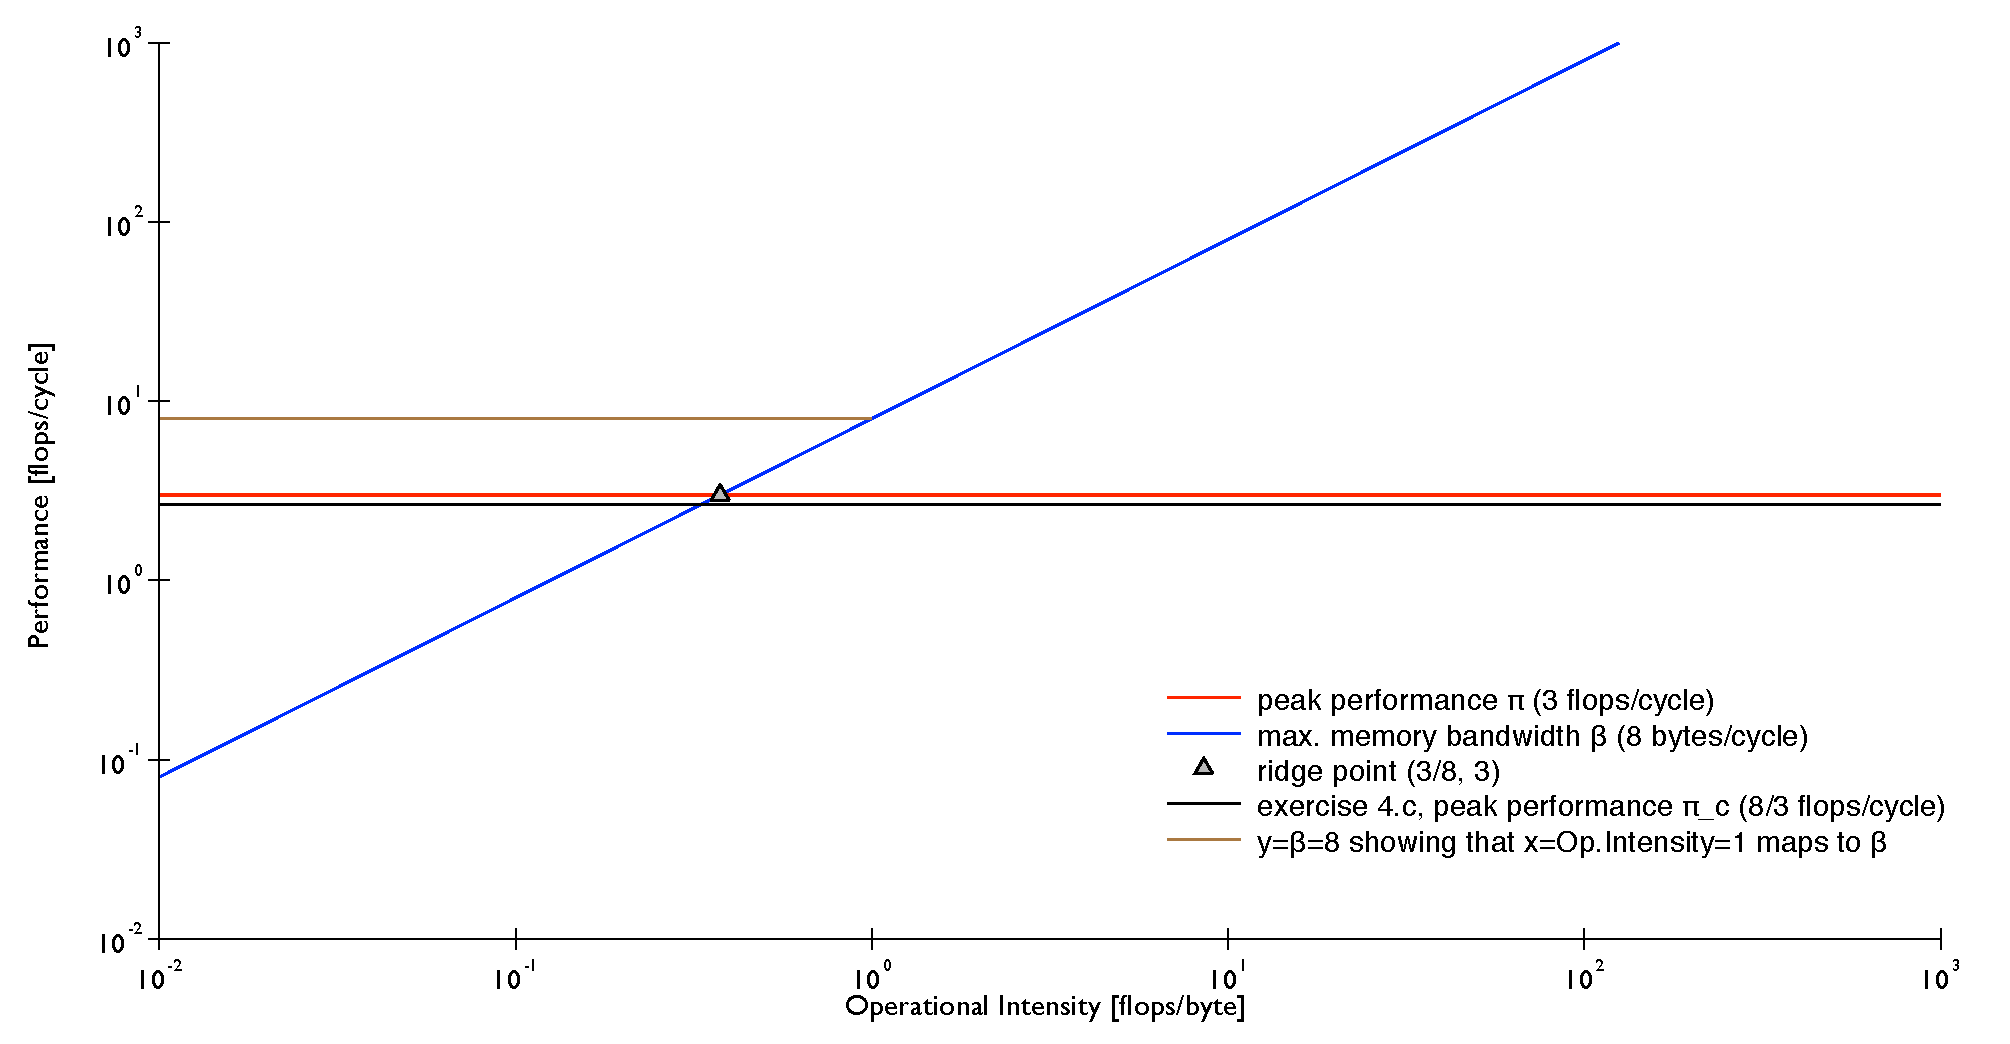
\includegraphics[height=13cm]{roofline}
\label{roofline_plot}
\end{figure}
\end{landscape}

\subsection*{(d)}
Aussuming N is sufficiently small such that the working set fits into cache ($3*N^3*4B<=8MB$) the peak performance can be reached. There are two multiplications and one addition which is exactly what our cpu can execute per cycle.
It should be noted that the first and last addition cannot be executed simultaneously to the other two multiplications because they depend on their result. But since it's just two operations out of the $3*N^3$ operations I'd say that peak performance can be reached.

\subsection*{(e)}
Yes, it's possible for compute3(A,B,C,65536) to reach peak performance. 
Som observations/assumptions:
\begin{itemize}
\item 16 floats fit into one cache block
\item loading one matrix column takes $16*4*65536=4MiB$
\item I assume that the ith column of A and the jth column of B are loaded to cache (and stay there).
\end{itemize}
The matrix \underline{A has to be loaded once}. The outer loop fixes the column and then it can be reused (since it's in cache) in the inner two loops.\\ The matrix \underline{B has to be loaded N times}. 4Mib of the cache are already used for the column of A. Since the column of B is set by the second loop it must therefore be read N times. \\
\underline{Each element of C has to be read only once}. Under the assumption that the ith column of A and the jth column of B is in cache, we know that the cache is full. This means that\\ \underline{for each element of C a whole cache block must be read}. Assuming that the block is invalidated afterwards and we have to fill this block again with data for the columns of A or B we have to read $2*64*N^2$ bytes to read the elements of C and 'restore' the block with the value from A or B.

This function has $W(n)=3*N^3$ and using the assumptions above\\ $Q(n)=4*N^2+4*N^3+2*64*N^2$ (A + N times B + C including overhead and restore) With $N=65536$ this gives an operational intensity of $\underline{I(n)=\frac{3*65536^3}{4*65536^2+4*65536^3+2*64*65536^2}=0.75}$
This is on the right side of the ridge point at $x=3/8=0.375$ and therefore compute bound. From exercise (d) we know that peak performance can therefore be reached.

\section*{Exercise 5 - Roofline and MMM}
\subsection*{(a)}
By definition we have: 
$I(n)=\frac{W(n)}{Q(n)}$ \\
Since the dot of the function lies on the ridge point we also know that
$T_{comp} = \frac{W(n)}{\pi}$  and
$T_{mem} = \frac{Q(n)}{\beta}$. \\
As seen in exercise four the ridge point lies on $x=\pi/\beta$ and $y=\pi$ and therefore $I(n)=\pi/\beta$ (x-Axis). \\
Starting with the definition of \\
$I(n)=\frac{W(n)}{Q(n)} \\
 \implies \frac{W(n)}{Q(n)} = \pi/\beta \\
  \implies \frac{W(n)}{\pi} = \frac{Q(n)}{\beta}\\
  \implies T_{comp} = T_{mem}$ what concludes the proof.

The reverse can also be shown by applying the above steps backwards. The reverse only holds under the assumption that $\pi, \beta$ and $Q(n)$ are $!=0$.
\subsection*{(b)}
\begin{itemize}
\item $W(N) = 2*N^3$
\item Minimal number of cache misses $\implies$ matrices are multiplied by blocks using an \underline{optimal} blocksize $N_B$ 
\item Dots lie on the ridge point $\implies I(n) = \pi/\beta$ 
\item From the lecture notes we know that for MMM the optimal achievable operational intensity lies in $\theta(sqrt(N))$
\item On the new cpu we have an operational intensity of $\frac{\pi'}{\beta}=\frac{\alpha*\pi}{\beta}$ (when the dots lie on the ridge point)
\end{itemize}
In the lecture we modelled the optimal block size using the formula $\ceil{\frac{N_B^2}{B_1}} + 3*\ceil{\frac{N_B}{B_1}} + 1 <= \frac{\gamma}{B_1}$ with $B_1$ being the cache block size. When multipliying by blocks for each block-multiplication we have to load three bocks (from matrix A, B and from the resulting matrix). This means $3*N^3$ elements are loaded per block-multiplication. There are $(N/N_B)^2$ blocks in a matrix and for each of those blocks we have $N/N_B$ block-multiplications resulting in $(N/N_B)^3$ block-multiplications.\\
$Q(n)={3*N^3 * (N/N_B)^3}=\frac{3*N^3}{N_B}$ \\ (elements per multiplication times number of block-multiplications) \\
Using this new $Q(n)$ and $W(n)$ from above the operational intensity becomes: \\ $I(n)=\frac{W(n)}{Q(n)}=\frac{2*N^3}{\frac{3*N^3}{N_B}} = \frac{2*N^3*N_B}{3*N^3} =\frac{\pi}{\beta}$
Knowing that the cpu has peak performance $\pi'=\alpha*\pi$ and that we want the dot to lie on the ridge point again we must have a computational intensity of $I(n)=\frac{\pi'}{\beta} = \frac{\alpha*\pi}{\beta}$. This can be achieved by using a new matrix-blocksize of $N_B'=N_B*\alpha$. \\
The new blocksize still needs to satisfy the inequality from the lecture. \\
$\ceil{\frac{N_B'^2}{B_1}} + 3*\ceil{\frac{N_B'}{B_1}} + 1 <= \frac{\gamma*\lambda}{B_1}$ \\
where $\lambda$ is a new introduced factor by which the cache size has to increase. \\
Replacing $N_B'$ with $N_B*\alpha$ leads to
$\ceil{\frac{N_B^2\alpha^2}{B_1}} + 3*\ceil{\frac{N_B*\alpha}{B_1}} + 1 <= \frac{\gamma*\lambda}{B_1}$ \\
So the factor $\lambda$ needs to be at least $\lambda>\alpha^2$ for the inequality to hold. The cache size must be increased by a factor of $O(\alpha^2)$.
\end{document}
